\subsection{Bohrsches Atommodell}
Das Bohrsche Atommodell beschreibt ein Atom, das aus einem positiv geladenen Kern und einer Hülle aus Elektronen besteht. Die Elektronen können sich dabei nur auf festgelegten geschlossenen Bahnen um den Kern bewegen. Auf den einzelnen Bahnen haben nur begrenzt viele Elektronen Platz, wobei alle Elektronen auf einer Bahn die gleiche Energie haben. Jeder Bahn wird also ein Energieniveau $E_i$ zugeordnet. \cite[Kap. 14.1.1]{Walcher}\\
Angenommen ein so aufgebautes Atom ist in Ruhe und trifft auf ein bewegtes Elektron. Sei $E_0$ das Niveau mit der niedrigsten Energie, $E_1$ das nächsthöhere und $\Delta E$ die Differenz zwischen den beiden. Abhängig von der kinetischen Energie des Elektrons $E_\text{kin}$ können zwei verschiedene Beobachtungen gemacht werden:
\begin{enumerate}
	\item $E_\text{kin}<\Delta E$: Elastischer Stoß. Das heißt es wird keine Energie (dauerhaft) übertragen. Da das Atom im Verhältnis zum Elektron sehr schwer ist, kann genähert werden, dass das Atom an seinen ursprünglichen Ort verbleibt und das Elektron die Richtung, nicht aber den Betrag seiner Geschwindigkeit verändert.
	\item $E_\text{kin}\geq\Delta E$: Inelastischer Stoß. Das Elektron hat genug Energie, um das Atom anzuregen. Das bedeutet, das Elektron überträgt die Energie $\Delta E$ auf das Atom, sodass ein Hüllenelektron von $E_0$ auf $E_1$ \grqq angehoben\grqq\ wird. Die kinetische Energie des bewegten Elektrons nach dem Stoß ist
	\begin{align}
		E_\text{kin,nach} &= E_\text{kin,vor} - \Delta E \ .
	\end{align}
	Für das Atom ist der angeregte Zustand instabiler, als der Grundzustand, weshalb das zuvor angehobene Elektronen nach kurzer Zeit wieder auf $E_0$ \grqq herunterfällt\grqq. Dabei wird ein Lichtquant emittiert, was auf Grund der Energieerhaltung genau die Energie
	\begin{align}\label{eq:energie1}
		h\nu = \Delta E
	\end{align}
	besitzt. $h$ ist das Plancksche Wirkungsquantum, $\nu$ die Frequenz des emittierten Lichts.
\end{enumerate}
Diese Prozesse können auf beliebige höhere, sowie nicht aufeinanderfolgende Niveaus verallgemeinert werden. Ganz speziell können noch ein beliebiges Niveau $E_i$ und das höchste Niveau $E_\text{max}$ mit der Energiedifferenz $\Delta E = E_\text{max}-E_i$ betrachtet werden. Hat das bewegte Elektron eine kinetische Energie, die größer ist, als $\Delta E$, dann wird ein Elektron aus der Atomhülle ausgelöst. Das Atom ist dann ionisiert. Die dafür nötige Energie wird als Ionisierungsenergie bezeichnet.
\clearpage

\subsection{Grundsätzlicher Aufbau}
Abbildung \ref{fig:AufbauSchematisch} zeigt den prinzipiellen Aufbau des Franck-Hertz-Versuchs. Der schraffierte Bereich ist ein evakuierter Glaskolben in dem sich Quecksilbergas befindet. Durch Glüh\-emission werden Elektronen aus dem Glühdraht emittiert. Durch die Beschleunigungsspannung $U_\text{B}$ werden die Elektronen beschleunigt. Dabei gilt allgemein der Zusammenhang
\begin{align}
	E_\text{kin} = eU \ ,
\end{align}
mit der Elementarladung $e$. Die Spannung $U$ ist die vom Elektron überwundene Spannungsdifferenz. \\
Treten nur elastische Stöße auf, haben die Elektronen an der Beschleunigungselektrode eine Geschwindigkeit von
\begin{align}
	v = \sqrt{\frac{2eU_\text{B}}{m}} \ ,
\end{align}
mit der Elektronenmasse $m$. Die Beschleunigungselektrode ist ein leitendes Gitter, sodass es Elektronen hindurch lässt, aber dennoch als Spannungspol verwendet werden kann. Je nachdem, ob die Bremsspannung $U_\text{A}$ positiv oder negativ ist, werden die Elektronen gebremst oder positiv beschleunigt und können, falls sie die Auffängerelektrode erreichen, als Strom $I_\text{A}$ gemessen werden.
\begin{figure}[h!]
	\centering
	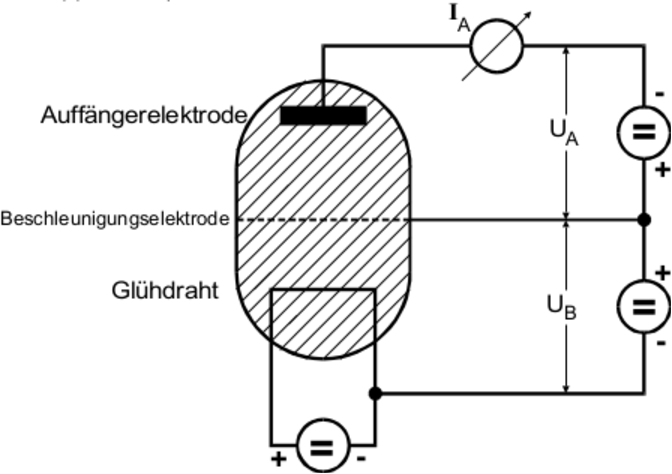
\includegraphics[width = 0.6\textwidth]{Aufbau_prinzipiell.pdf}
	\caption{Schematischer Aufbau des Frank-Hertz-Versuchs \cite{\V}}
	\label{fig:AufbauSchematisch}
\end{figure} \\
Sei die Bremsspannung konstant und klein. Wird $U_\text{B}$, beginnend bei $U_\text{B}=\SI{0}{\volt}$, erhöht, wird ein Strom gemessen, sobald die Elektronen das geringe Gegenfeld überwinden können. Ist die Spannung dann gerade
\begin{align}\label{eq:energie2}
	eU_\text{B} = \Delta E 
\end{align}
($\Delta E$ ist wie im vorigen Abschnitt die Anregungsenergie), fällt der Strom abrupt ab, da die Elektronen kurz vor der Beschleunigungselektrode inelastisch mit den Atomen stoßen und danach keine kinetische Energie mehr haben, um das Gegenfeld zu überwinden. Wird die Beschleunigungsspannung weiter erhöht, können die Elektronen immer früher ihre kinetische Energie abgeben. Da sie dann aber noch nicht bei der Beschleunigungselektrode sind, werden sie wieder beschleunigt und können wieder als Strom detektiert werden. Sobald für $U_\text{B}$ gilt
\begin{align}
	2eU_\text{B} = \Delta E
\end{align}
kann ein zweiter inelastischer Stoß der Elektronen mit den Atomen statt finden, usw.